\documentclass[11pt]{article}
\headheight=13.6pt

% packages
\usepackage{amsfonts, amsmath, amssymb, amsthm}
% margin spacing
\usepackage[top=1in, bottom=1in, left=0.5in, right=0.5in]{geometry}
\usepackage{hanging}
\usepackage{fancyhdr}
\usepackage{graphicx}
\graphicspath{{./images/}}
%\usepackage{siunitx}
\usepackage{enumitem}
\usepackage{hyperref}
\hypersetup{colorlinks=true,urlcolor=blue}
\usepackage{textcomp}

% header/footer formatting
\pagestyle{fancy}
\fancyhead{}
\fancyfoot{}
\fancyhead[L]{CDA3101}
\fancyhead[C]{Cache Simulation Analysis Paper}
\fancyhead[R]{Sai Sivakumar}
\fancyfoot[R]{\thepage}
\renewcommand{\headrulewidth}{1pt}

% paragraph indentation/spacing
\setlength{\parindent}{0cm}
\setlength{\parskip}{10pt}
\renewcommand{\baselinestretch}{1.25}

% smileys frownies
\usepackage{wasysym}
\newcommand{\happy}{\raisebox{-.28em}{\resizebox{1.5em}{!}{\smiley}}}
\newcommand{\darkhappy}{\raisebox{-.28em}{\resizebox{1.5em}{!}{\blacksmiley}}}
\newcommand{\sad}{\raisebox{-.28em}{\resizebox{1.5em}{!}{\frownie}}}

% functions
\newcommand{\fn}[1]{\texttt{#1}}

% pink p and colorbox
\usepackage{xcolor}
\definecolor{p}{HTML}{FFDDDD}
\usepackage[skins]{tcolorbox}
\newtcbox\leftbox{hbox, on line, colback=p, enhanced, frame hidden, boxrule=0pt, 
    top=0pt, bottom=0pt, right=-3pt, left=-3pt, sharp corners}

% set page count index to begin from 1
\setcounter{page}{1}

\begin{document}
\begin{enumerate}[left= \parindent, label = \textbf{\arabic*.}]
    \item \textbf{Introduction}
    
    In this paper we analyze the hit rate of cache designs as the configuration for the cache is changed. Specifically, we vary the cache size (with fixed size of lines in the cache), set associativity, and the replacement policy of the cache and inspect the corresponding hit rates for trends. The goal of this paper is to investigate and understand the performance impacts of changing the above parameters, specifically the hit rate as opposed to other performance metrics like access time or insertion rate (e.g. for access time, these values would differ amongst devices).
    \item \textbf{Testing Procedure}
    
    We run seven tests, each varying the cache size, followed by varying the set associativity of the cache, and lastly the cache's replacement policy where applicable. To vary the cache size, we vary the number of lines in the cache while fixing the size of each line to $16$ bytes per line. So the size of the cache is given by $16x = 2^42^{\log_2(x)} = 2^{4+\log_2(x)}$, where $x$ is the number of lines per cache, and we consider $x\in \{128, 256, 512, 1024, 2048, 4096\}$ so that the cache size in bytes is an element of $\{2^{11},2^{12},2^{13},2^{14},2^{15},2^{16}\}$. Obtain the following seven tests as functions of $x$ (where $x\in \{128, 256, 512, 1024, 2048, 4096\}$):
    \begin{center}
        \begin{tabular}[h]{|c|c|c|c|}
            \hline\textbf{Test} & \textbf{Cache Size (bytes)} & \textbf{Set Associativity} & \textbf{Replacement Policy}\\            
            \hline $1$& $16x$& Full. Assoc.& LRU\\
            \hline $2$& $16x$& Full. Assoc.& FIFO\\
            \hline $3$& $16x$& $2$-Way Set Assoc.& LRU\\
            \hline $4$& $16x$& $2$-Way Set Assoc.& FIFO\\
            \hline $5$& $16x$& $8$-Way Set Assoc.& LRU\\
            \hline $6$& $16x$& $8$-Way Set Assoc.& FIFO\\
            \hline $7$& $16x$& Direct Mapped& Not Applicable\\
            \hline
        \end{tabular}
    \end{center}
    Each test computes the hit rate of a fixed set of data requests of a cache type above given the number of lines per cache $x$ (note varying the number of lines per cache varies the size of the cache linearly, since we have fixed the size of each line). We run one test via the provided program for each combination of cache size, set associativity, and replacement policy, and plot the hit rates against the number of lines $x$. We choose a couple types of set associativity aside from fully associative and direct mapped to make a gradual change from fully associative to direct mapping set schemes, and we increase the number of lines per cache by powers of two to gradually (exponentially) increase the capacity of the cache to investigate how short-term and long-term growth of the cache size affects performance.
    \item \textbf{Results}
    
    The data for hit rates against count of lines in cache:
    \begin{center}
        \begin{tabular}[h]{|c|c|c|c|c|c|c|c|}
            \hline\textbf{\#Lines\textbackslash Test} & $1$ & $2$ & $3$ & $4$ & $5$ & $6$ & $7$\\            
            \hline $128$ & $0.964449$ & $0.954965
            $ & $0.935288$ & $0.928861
            $ & $0.961971
            $ & $0.953481
            $ & $0.890858
            $\\
            \hline $256$ & $0.971093
            $ & $0.965714
            $ & $0.962095$ & $0.957804
            $ & $0.970135
            $ & $0.965213
            $ & $0.938687
            $\\
            \hline $512$ & $0.974186
            $ & $0.971479
            $ & $0.971213$ & $0.969163
            $ & $0.974025
            $ & $0.971223
            $ & $0.958387
            $\\
            \hline $1024$ & $0.975935
            $ & $0.974296
            $ & $0.974585
            $ & $0.97323
            0$ & $0.975766
            $ & $0.974124
            $ & $0.969084
            $\\
            \hline $2048$ & $0.977046
            $ & $0.976249
            $ & $0.976464
            $ & $0.975648
            $ & $0.976906
            $ & $0.976075
            $ & $0.972894
            $\\
            \hline $4096$ & $0.97761
            0$ & $0.977195
            $ & $0.97729
            0$ & $0.97687
            0$ & $0.977539$ & $0.977075
            $ & $0.975547
            $\\
            \hline
        \end{tabular}
    \end{center}
    The corresponding plot of the data:
    
    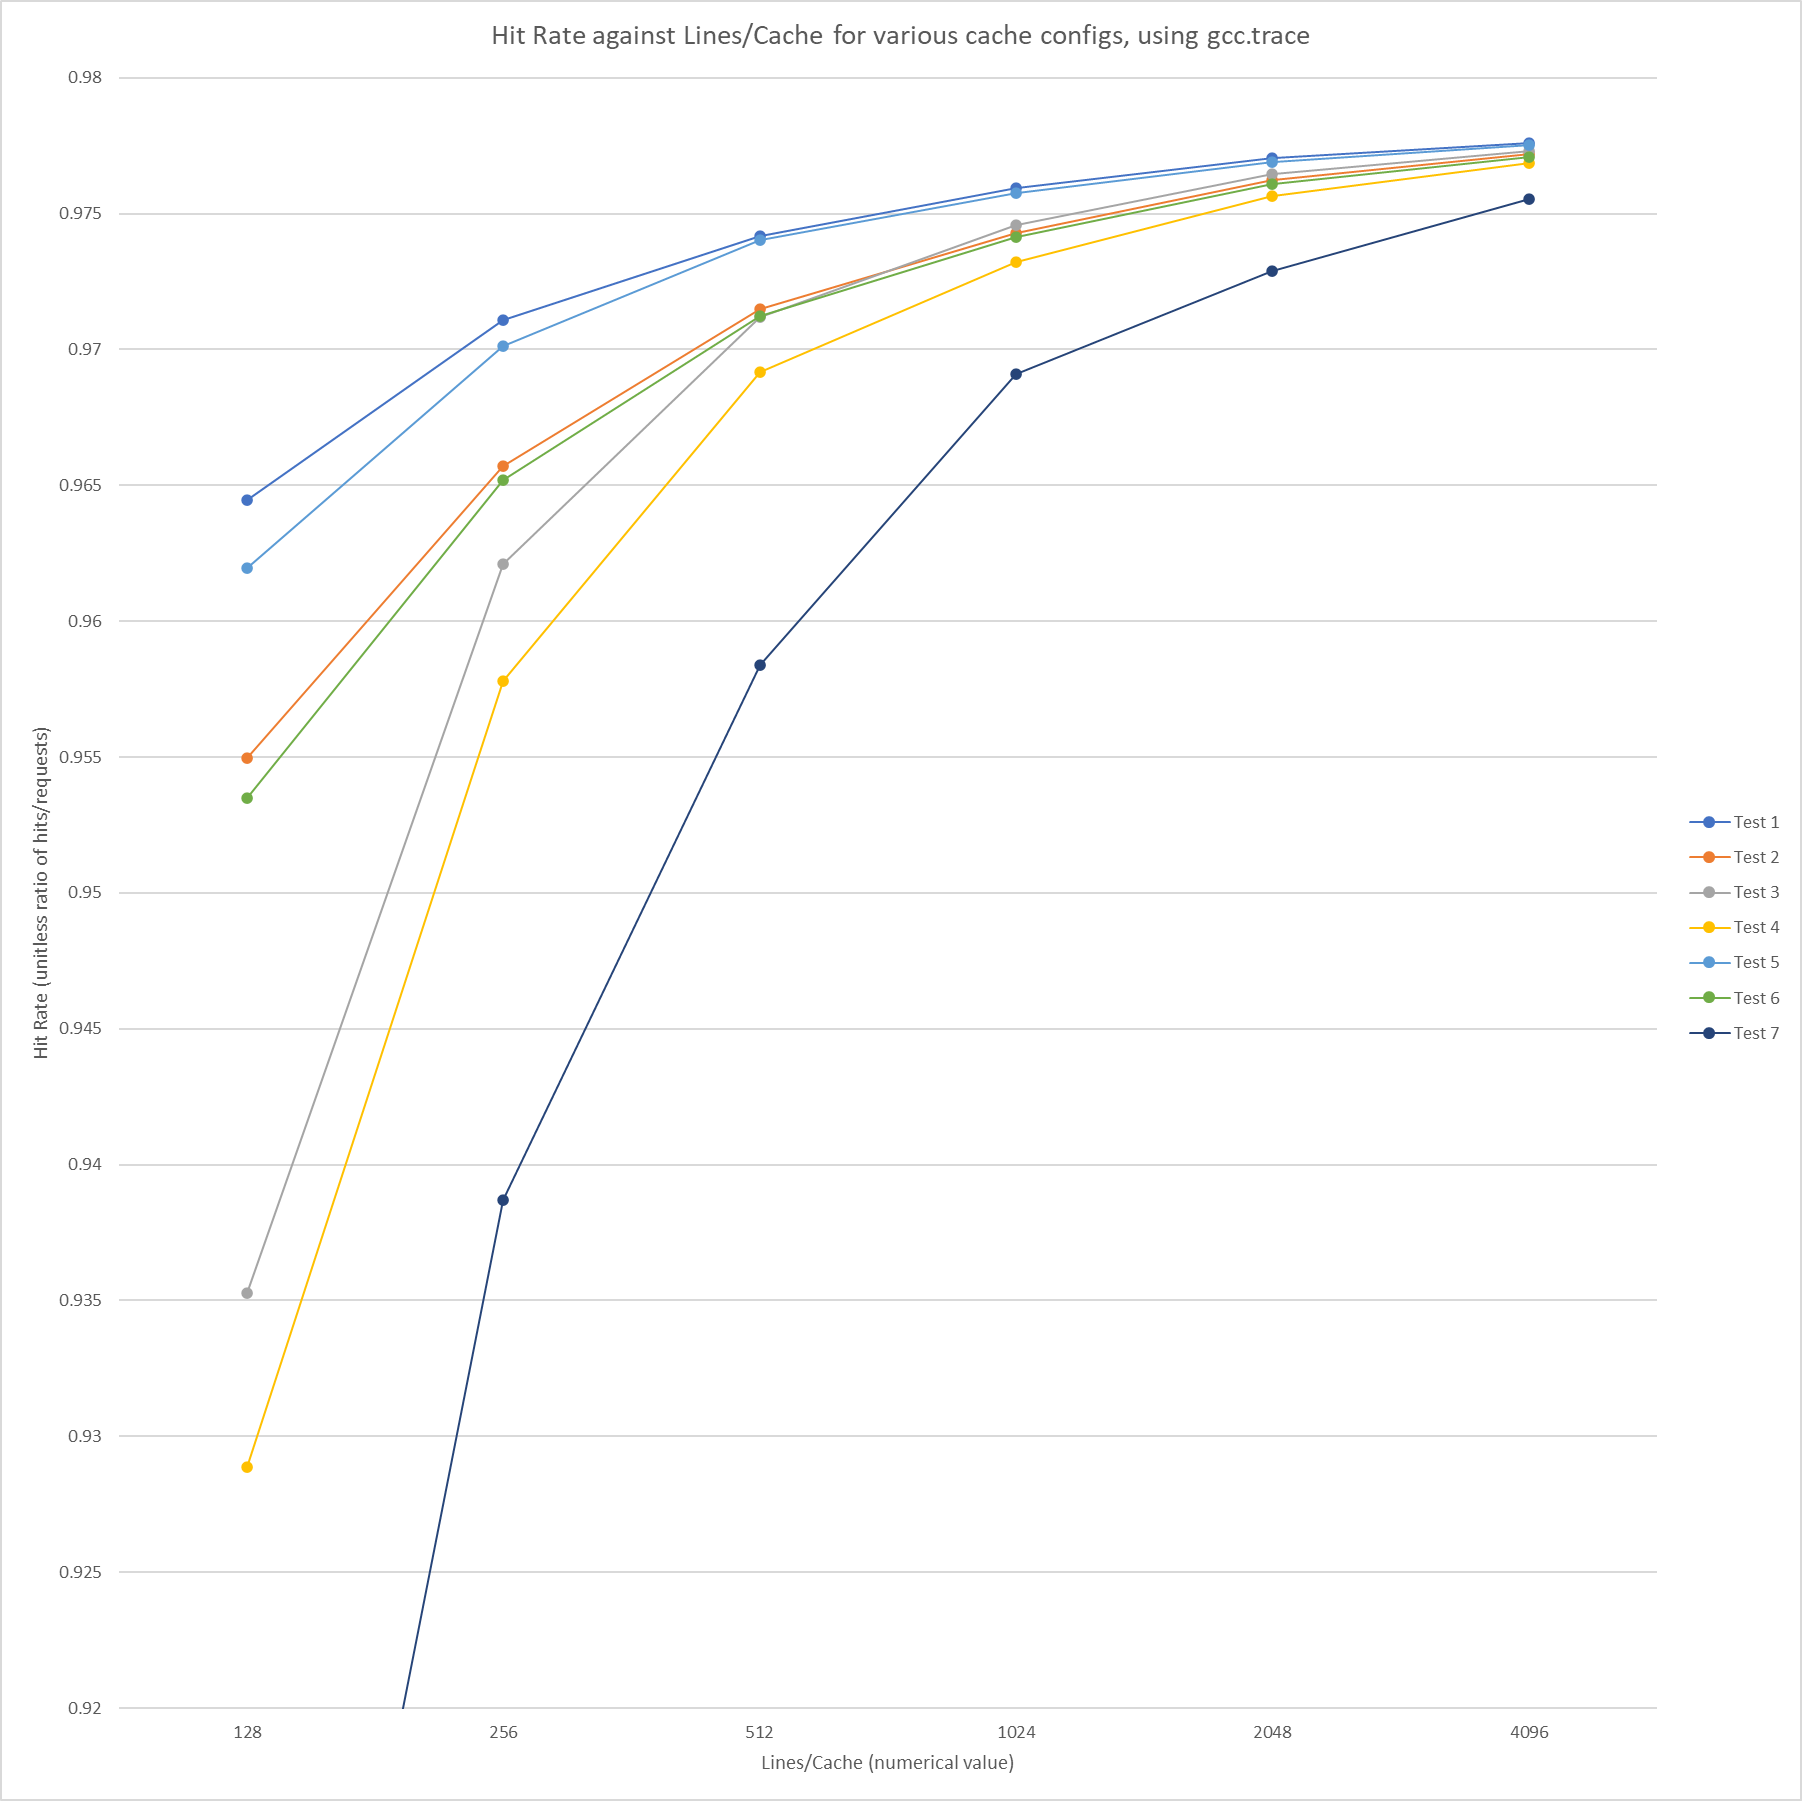
\includegraphics[scale=.37]{data.png}
    \item \textbf{Conclusion}
    
    It is evident that increasing the size of the cache will improve the hit rate for the cache: More data can be stored on the cache without replacement, so any requested data would have a higher probability of remaining on the cache, yielding an increased hit rate.

    Now considering just the cache design, the data suggests that the fully associative cache has a higher hit rate than the $8$-way set associative cache, followed by the $2$-way associative cache and then the direct mapped cache. This is reasonable since for the fully associative cache, any block from memory can be placed in any line in the cache, utilizing the cache space effectively. This is in contrast with $m$-way set associative caches that have to store blocks from memory in specific places (and the specificity increases as $m$ decreases), which will lead to many unutilized lines as well as data being replaced in the cache when space could have been used. This phenomenon causes the set associative caches as well as the direct mapped cache to suffer in hit rate.
    
    Then comparing the LRU and FIFO replacement policies, it seems that in all cases the tests with LRU replacement policy had a higher hit rate than the corresponding FIFO cache test. This is expected since FIFO caches indiscriminately replace data, even if said data were requested frequently, leading to a decreased hit rate. Conversely, the LRU replacement policy replaced the least recently used line from the cache, which would improve the hit rate since more frequently requested data would remain in the cache for quick access.
\end{enumerate}
\end{document}